% Provenance (never printed): see sources/outline_sources.md (Year 1:
% astronomy of position, spherical trigonometry, time scales, insolation).
% Spherical trigonometry is absent from the mathematics series: this chapter
% owns it. Curves computed in figdata/bachelor-1/{sun_paths, day_length,
% celestial_sphere, spherical_triangle}.py (shared model _solar.py); numbers
% of the exercises and problem in the Book 3 scratch calculator ch01.py.
\chapter{球面天文学}\label{ch:b1:spherical-astronomy}

在远离城镇、天空晴朗的夜晚，一台对准天空的长曝光照相机
记录下的恒星呈一段段圆弧，它们都以同一个
不动的点为圆心。今晚九点从东方升起的恒星，明天将
约在九点差五分升起，此后每晚都提早一些。正午时的太阳
六月比十二月更高，在遥远的北方，它
仲夏时整日不落。这一切都是地球自转
及其绕太阳公转的结果，从地面看去。为了描述它们，天文学家
与地球科学家需要球面上的坐标、
\omterm{def:b1:spherical-astronomy:spherical-triangle}{球面三角形}的三角学，以及与恒星或太阳同步的时钟。
本章建立这些工具。它们将在
板块运动学（\cref{ch:b1:plate-kinematics}）中再次出现，那里板块在
球面上转动；也在气候各章（\cref{ch:b1:radiation-heat-transport}）中出现，
那里某一\omterm{def:b1:spherical-astronomy:geographic}{纬度}所接收的日照驱动着风与洋流。

\begin{recall}
地球每天绕自转轴转动一周，
每年沿近似圆形的轨道绕太阳公转一周；其自转轴相对轨道面倾斜，
从而形成季节（见物理系列的六年级与十二年级分册；
开普勒定律已在物理系列的本科一年级分册中回顾）。
地球上一点由\omterm{def:b1:spherical-astronomy:geographic}{纬度}和\omterm{def:b1:spherical-astronomy:geographic}{经度}确定（第 1 册，六年级）。
长度为 1 的矢量由两个角确定，如球坐标中所示；
两个单位矢量的点积等于它们夹角的余弦，混合积
$\vec u\cdot(\vec v\times\vec w)$ 在三个矢量的轮换置换下
保持不变。
\end{recall}

\section{球面三角形}

\begin{definition}[大圆、球面三角形]\label{def:b1:spherical-astronomy:spherical-triangle}
球面的\emph{大圆}\index{大圆}是球面与过球心的平面的交线；
其他任何平面的截面称为
\emph{小圆}\index{小圆}。过不互为对径的两点
恰有一个大圆，两段弧中较短者即为两点间球面上的最短路径。
由球面上三点构成的图形称为\emph{球面三角形}\index{球面三角形}，
其顶点为 $A$、$B$、$C$，三边为两两相连的大圆弧，
每段弧都小于 \ang{180}。
其边 $a$、$b$、$c$ 分别与顶点 $A$、$B$、$C$ 相对，
以其在球心所张的角度量；其角 $A$、$B$、$C$
为各顶点处两条相交边所在平面之间的夹角。
\end{definition}

在半径为 $R$ 的球面上，弧度为 $a$ 的边长为 $Ra$。每条
边与每个角都介于 $0$ 与 $\pi$ 之间。

\begin{omfigure}
\begin{tikzpicture}
\begin{axis}[x=1cm, y=1cm, hide axis, xmin=-2.7, xmax=2.7, ymin=-2.6, ymax=2.6, clip=false]
\draw[black, line width=0.6pt] (axis cs:0,0) circle (2.4cm);
\addplot[black!45, densely dashed, line width=0.4pt] coordinates {(0,0) (-0.078358,1.7847)};
\addplot[black!45, densely dashed, line width=0.4pt] coordinates {(0,0) (-1.5903,-0.2902)};
\addplot[black!45, densely dashed, line width=0.4pt] coordinates {(0,0) (1.4453,-0.16381)};
\addplot[omDef, line width=1.1pt] table {figdata/out/bachelor-1-spherical_triangle-ab.dat};
\addplot[omDef, line width=1.1pt] table {figdata/out/bachelor-1-spherical_triangle-bc.dat};
\addplot[omDef, line width=1.1pt] table {figdata/out/bachelor-1-spherical_triangle-ca.dat};
\addplot[omThm, line width=0.8pt] table {figdata/out/bachelor-1-spherical_triangle-angA.dat};
\addplot[only marks, mark=*, mark size=1.4pt] table[x=x, y=y] {figdata/out/bachelor-1-spherical_triangle-verts.dat};
\fill (axis cs:0,0) circle (1.2pt);
\begin{scope}[font=\small]
  \node[above] at (axis cs:-0.078358,1.7847) {$A$};
  \node[left] at (axis cs:-1.5903,-0.2902) {$B$};
  \node[right] at (axis cs:1.4453,-0.16381) {$C$};
  \node[above left] at (axis cs:0,0) {$O$};
  \node[omThm] at (axis cs:0.24,1.36) {$A$};
  \node[omDef] at (axis cs:0.0,-0.52) {$a$};
  \node[omDef] at (axis cs:0.95,0.95) {$b$};
  \node[omDef] at (axis cs:-1.05,0.95) {$c$};
\end{scope}
\end{axis}
\end{tikzpicture}

{\small \omterm{def:b1:spherical-astronomy:spherical-triangle}{球面三角形} $ABC$ 位于球心为 $O$ 的球面上。边 $a$、
$b$、$c$ 为\omterm{def:b1:spherical-astronomy:spherical-triangle}{大圆}弧，分别由角 $BOC$、$COA$、
$AOB$ 度量；角 $A$（红色）为在
$A$ 处相交两边之间的夹角。图中三角形的边为 $a = \ang{78.6}$、$b = \ang{62.6}$、
$c = \ang{64.8}$，三个角分别为 \ang{89.9}、\ang{64.9} 和 \ang{67.4}，
它们之和大于 \ang{180}。}
\end{omfigure}

\begin{theorem}[余弦定理]\label{thm:b1:spherical-astronomy:cosine-rule}
在\omterm{def:b1:spherical-astronomy:spherical-triangle}{球面三角形}中，
\[
  \cos a = \cos b\cos c + \sin b\sin c\cos A .
\]
\end{theorem}

\begin{proof}
在单位球面上取坐标轴，使 $A$ 位于极点：
$\vec A = (0, 0, 1)$，并取平面 $xz$，使其包含 $B$：
$\vec B = (\sin c, 0, \cos c)$，因为 $B$ 的角距离为 $c$
（自 $A$ 量起）。点 $C$ 的角距离为 $b$（自 $A$ 量起），位于一个
过 $A$ 的\omterm{def:b1:spherical-astronomy:spherical-triangle}{大圆}上，该\omterm{def:b1:spherical-astronomy:spherical-triangle}{大圆}以角 $A$ 倾斜于平面 $xz$：
$\vec C = (\sin b\cos A, \sin b\sin A, \cos b)$。边 $a$ 为
$\vec B$ 与 $\vec C$ 之间的夹角，于是
\[
  \cos a = \vec B\cdot\vec C = \sin c\sin b\cos A + \cos c\cos b. \qedhere
\]
\end{proof}

\begin{theorem}[正弦定理]\label{thm:b1:spherical-astronomy:sine-rule}
在\omterm{def:b1:spherical-astronomy:spherical-triangle}{球面三角形}中，
\[
  \frac{\sin A}{\sin a} = \frac{\sin B}{\sin b} = \frac{\sin C}{\sin c}.
\]
\end{theorem}

\begin{proof}
沿用前一证明中的向量，
$\vec B \times \vec C = (-\cos c\sin b\sin A,\allowbreak\ \cos c\sin b\cos A - \sin c\cos b,\allowbreak\
\sin c\sin b\sin A)$，故三重积为
$\vec A\cdot(\vec B\times\vec C) = \sin b\sin c\sin A$。三重积
在 $A$、$B$、$C$ 循环置换下保持不变；依次将 $B$、$C$ 置于极点，
同理得 $\sin c\sin a\sin B$ 与 $\sin a\sin b\sin
C$。三式相等，两边除以 $\sin a\sin b\sin c$ 得
正弦定理。
\end{proof}

边长与半径相比很小时，$\cos a \approx 1 -
a^2/2$，$\sin a \approx a$，两条规则化为平面三角形的余弦与
正弦定理：在足够小的局部上，球面近似为平面。对于
大三角形则不然：\omterm{def:b1:spherical-astronomy:spherical-triangle}{球面三角形}的三内角之和大于
\ang{180}（见\cref{exo:b1:spherical-astronomy:12}）。

\begin{method}[球面上的距离与方位]\label{met:b1:spherical-astronomy:great-circle}
求\omterm{def:b1:spherical-astronomy:geographic}{纬度}分别为 $\varphi_1$、
$\varphi_2$、\omterm{def:b1:spherical-astronomy:geographic}{经度}分别为 $\lambda_1$、$\lambda_2$ 的两地间的最短距离及
出发时的方向：
\begin{enumerate}
  \item 以北极 $P$ 与两地为顶点构成三角形；
        其从极点出发的两边为余纬 $\ang{90} -
        \varphi_1$ 与 $\ang{90} - \varphi_2$，其在极点处的角为
        \omterm{def:b1:spherical-astronomy:geographic}{经度}差 $\Delta\lambda$；
  \item 由余弦定理得角距离 $\Delta$：
        $\cos\Delta = \sin\varphi_1\sin\varphi_2 +
        \cos\varphi_1\cos\varphi_2\cos\Delta\lambda$；距离为
        $R\Delta$（$\Delta$ 以弧度计）；
  \item 初始方向即为三角形在第一地点处的角，
        由对该角之对边应用余弦定理求得，
        $\sin\varphi_2 = \sin\varphi_1\cos\Delta + \cos\varphi_1\sin\Delta\cos
        \mathrm{Az}$，自北向第二地点量取。
\end{enumerate}
沿\omterm{def:b1:spherical-astronomy:spherical-triangle}{大圆}\omterm{def:b1:spherical-astronomy:horizontal}{方位角}会发生变化（沿经线或
赤道除外）：保持罗盘方位不变的船只或飞机，
所走的是另一条更长的曲线。
\end{method}

\section{球面上的坐标}

\begin{definition}[纬度与经度]\label{def:b1:spherical-astronomy:geographic}
设地球为绕其极轴旋转的球体。
一点的\emph{纬度}\index{纬度} $\varphi$ 是过该点的半径与
赤道面之间的夹角，从 \ang{-90}
（南极）到 \ang{+90}（北极）；其\emph{经度}\index{经度}
$\lambda$ 是在赤道面内量得的该点子午半平面与
参考子午线的子午半平面之间的夹角，此参考子午线即
过格林尼治的子午线，向东为正，取值为 \ang{-180} 到
\ang{180}。
\end{definition}

事实上地球略呈扁平状；用于地图和天象的\omterm{def:b1:spherical-astronomy:geographic}{纬度}
为当地铅垂线与赤道面之间的夹角，
它与地心\omterm{def:b1:spherical-astronomy:geographic}{纬度}的差异至多为 \ang{0.2}
（见\cref{ch:b1:isostasy-gravity}）。纬线（即等纬线）是
\omterm{def:b1:spherical-astronomy:spherical-triangle}{小圆}；经线是\omterm{def:b1:spherical-astronomy:spherical-triangle}{大圆}的一半。

\begin{definition}[天球]\label{def:b1:spherical-astronomy:celestial-sphere}
\emph{天球}\index{天球}是以观测者为中心的假想球面，
每颗恒星都按其方向置于其上；只有
方向有意义，距离不计。地轴的延长线与天球相交于
北、南两\emph{天极}\index{天极}；
地球赤道面沿\emph{天
赤道}\index{天赤道}。\emph{天顶}\index{天顶}是
正上方、沿当地铅垂线方向的点；地平线是
距其 $\ang{90}$ 的\omterm{def:b1:spherical-astronomy:spherical-triangle}{大圆}。\emph{当地子午圈}\index{当地子午圈}是
过天顶与天极的\omterm{def:b1:spherical-astronomy:spherical-triangle}{大圆}；它与
地平线交于北点与南点。
\end{definition}

地球自西向东自转时，\omterm{def:b1:spherical-astronomy:celestial-sphere}{天球}看似
反向转动，自东向西，绕\omterm{def:b1:spherical-astronomy:celestial-sphere}{天极}连线旋转，约
一天略少的时间转一圈。恒星彼此的相对位置保持不变：它们
距离如此遥远，地球绕太阳公转一年，其方向的改变
不足一角秒（见\cref{ch:b1:observing-the-sky}）。

\begin{definition}[地平坐标]\label{def:b1:spherical-astronomy:horizontal}
恒星的\emph{海拔}\index{海拔（恒星）} $h$ 是其在地平线以上的
角度，取值从 \ang{-90} 到 \ang{90}；其\omterm{def:b1:spherical-astronomy:celestial-sphere}{天顶}距为
$z = \ang{90} - h$。其\emph{方位角}\index{方位角} $\mathrm{A}$ 为
沿地平线，自北点到恒星竖直圈的垂足所夹的角，
从 \ang{0} 计至 \ang{360}，经东方计量。
\end{definition}

地平坐标属于观测者，它随地点和
时间而变。\omterm{def:b1:spherical-astronomy:celestial-sphere}{天球}本身的坐标则随其转动而一同移动。

\begin{definition}[赤道坐标]\label{def:b1:spherical-astronomy:equatorial}
恒星的\emph{赤纬}\index{赤纬（天球）} $\delta$ 是其与\omterm{def:b1:spherical-astronomy:celestial-sphere}{天赤道}的夹角，
向北为正，取值从 \ang{-90}
到 \ang{90}。过恒星与\omterm{def:b1:spherical-astronomy:celestial-sphere}{天极}的\omterm{def:b1:spherical-astronomy:spherical-triangle}{大圆}是其
时圈。恒星的\emph{时角}\index{时角} $H$ 为
\omterm{def:b1:spherical-astronomy:celestial-sphere}{当地子午圈}与\omterm{def:b1:spherical-astronomy:sidereal-time}{恒星时}圈在\omterm{def:b1:spherical-astronomy:celestial-sphere}{天极}处所夹的角，
向西计量，以每 \ang{15} 为一小时。\emph{赤
经}\index{赤经} $\alpha$ 是沿\omterm{def:b1:spherical-astronomy:celestial-sphere}{天赤道}，自天空的一个固定点
即\omterm{def:b1:spherical-astronomy:ecliptic}{春分点}起算，量至\omterm{def:b1:spherical-astronomy:sidereal-time}{恒星时}圈所夹的角，
（见\cref{def:b1:spherical-astronomy:ecliptic}），
同样向东计量，同样以小时计。
\end{definition}

\omterm{def:b1:spherical-astronomy:equatorial}{赤纬}与\omterm{def:b1:spherical-astronomy:equatorial}{赤经}在\omterm{def:b1:spherical-astronomy:celestial-sphere}{天球}上是固定的，正如\omterm{def:b1:spherical-astronomy:geographic}{纬度}与
\omterm{def:b1:spherical-astronomy:geographic}{经度}在地球上那样：星表会列出它们。“\omterm{def:b1:spherical-astronomy:equatorial}{赤纬}”一词在此仅
取天文学意义；地理北与
指南针所指北方之间的夹角，一律称为磁偏角
（见\cref{ch:b1:field-lab-methods-1}）。

\begin{proposition}[由赤道坐标到地平坐标]\label{prop:b1:spherical-astronomy:transform}
在\omterm{def:b1:spherical-astronomy:geographic}{纬度} $\varphi$ 处，\omterm{def:b1:spherical-astronomy:equatorial}{赤纬}为 $\delta$、\omterm{def:b1:spherical-astronomy:equatorial}{时角}为 $H$ 的恒星，
其\omterm{def:b1:spherical-astronomy:horizontal}{海拔}与\omterm{def:b1:spherical-astronomy:horizontal}{方位角}由下式给出：
\[
  \sin h = \sin\varphi\sin\delta + \cos\varphi\cos\delta\cos H,
  \qquad
  \cos\mathrm{A} = \frac{\sin\delta - \sin\varphi\sin h}{\cos\varphi\cos h},
\]
$\mathrm{A}$ 取 \ang{0} 与 \ang{180} 之间的值，此时恒星位于子午线以东
（$\sin H < 0$）；$\mathrm{A} = \ang{360} - \arccos(\dots)$ 则对应
恒星位于西侧的情形。特别地，北\omterm{def:b1:spherical-astronomy:celestial-sphere}{天极}的\omterm{def:b1:spherical-astronomy:horizontal}{海拔}
等于\omterm{def:b1:spherical-astronomy:geographic}{纬度}。
\end{proposition}

\begin{proof}
考虑由北\omterm{def:b1:spherical-astronomy:celestial-sphere}{天极} $P$、\omterm{def:b1:spherical-astronomy:celestial-sphere}{天顶} $Z$
与恒星 $X$ 构成的三角形（天文三角形，又称位置三角形）。当地
竖直方向与赤道面成角 $\varphi$，故 $PZ =
\ang{90} - \varphi$；$PX = \ang{90} - \delta$；$ZX = \ang{90} - h$。在
$P$ 处的角为\omterm{def:b1:spherical-astronomy:equatorial}{时角} $H$；$Z$ 处的角为恒星的\omterm{def:b1:spherical-astronomy:horizontal}{方位角}，
自北（子午线以东或以西）量起。由余弦定理，
对边 $ZX$，其对角为 $P$，得
$\cos(\ang{90} - h) = \cos(\ang{90} - \varphi)\cos(\ang{90} - \delta) +
\sin(\ang{90} - \varphi)\sin(\ang{90} - \delta)\cos H$，即第一式。
由余弦定理，对边 $PX$，其对角为 $Z$，得
$\sin\delta = \sin\varphi\sin h + \cos\varphi\cos h\cos\mathrm{A}$，即第二式。
对于\omterm{def:b1:spherical-astronomy:celestial-sphere}{天极}，$\delta = \ang{90}$，第一式化为
$\sin h = \sin\varphi$。
\end{proof}

\begin{omfigure}
\begin{tikzpicture}
\pic (cs) at (0,0) {celestialsphere=45};
\begin{axis}[x=1cm, y=1cm, hide axis, anchor=origin, at={(0,0)}, xmin=-2.6, xmax=2.6, ymin=-2.4, ymax=2.5, clip=false]
\addplot[omField, line width=1.1pt] table[x=x, y=y] {figdata/out/bachelor-1-celestial_sphere-vertical.dat};
\addplot[black!80, line width=0.9pt, densely dash dot] table[x=x, y=y] {figdata/out/bachelor-1-celestial_sphere-hourcircle.dat};
\addplot[only marks, mark=star, mark size=3pt, mark options={line width=0.8pt}] table[x=x, y=y] {figdata/out/bachelor-1-celestial_sphere-star.dat};
\end{axis}
\begin{scope}[font=\footnotesize]
  \node[above] at (cs-Z) {$Z$};
  \node[above left] at (cs-NCP) {$P$};
  \node[left] at (cs-N) {北};
  \node[right] at (cs-S) {南};
  \node[below] at (cs-W) {西};
  \node[below, fill=white, fill opacity=0.8, text opacity=1, inner sep=1pt] at (cs-E) {东};
  \node[above right] at (0.2262,0.94) {$X$};
  \node[omField] at (0.55,0.2) {$h$};
  \node[omDef, right] at (2.0,-1.25) {赤道};
  \node[left] at (-2.0,-0.3) {地平线};
  \node at (-1.35,0.62) {$\varphi$};
\end{scope}
\draw[black!60, line width=0.4pt] (-1.05,0) arc[start angle=180, end angle=137, radius=1.05cm];
\end{tikzpicture}

{\small 北纬 \ang{45} 处的天空，自西向望，北在左侧。
北\omterm{def:b1:spherical-astronomy:celestial-sphere}{天极} $P$ 的\omterm{def:b1:spherical-astronomy:horizontal}{海拔}等于
\omterm{def:b1:spherical-astronomy:geographic}{纬度}，位于北点上方（红色：\omterm{def:b1:spherical-astronomy:celestial-sphere}{天极}轴）；
\omterm{def:b1:spherical-astronomy:celestial-sphere}{天赤道}（蓝色）与
地平线在东、西两点相交。一颗\omterm{def:b1:spherical-astronomy:equatorial}{赤纬}为 \ang{25} 的恒星 $X$，
过子午线后三小时二十分（\omterm{def:b1:spherical-astronomy:equatorial}{时角}
\ang{50}），其\omterm{def:b1:spherical-astronomy:horizontal}{海拔}为 $h = \ang{45.3}$（绿色：其竖直圈，
自\omterm{def:b1:spherical-astronomy:celestial-sphere}{天顶} $Z$ 至地平线），\omterm{def:b1:spherical-astronomy:horizontal}{方位角}为 \ang{261}；其时圈
（点划线）自\omterm{def:b1:spherical-astronomy:celestial-sphere}{天极}经恒星至\omterm{def:b1:spherical-astronomy:celestial-sphere}{天赤道}。
由\cref{prop:b1:spherical-astronomy:transform}算得。}
\end{omfigure}

\begin{proposition}[中天与拱极星]\label{prop:b1:spherical-astronomy:culmination}
在\omterm{def:b1:spherical-astronomy:geographic}{纬度} $\varphi$ 处，\omterm{def:b1:spherical-astronomy:equatorial}{赤纬}为 $\delta$ 的恒星
于子午线上中天（$H = 0$）时\omterm{def:b1:spherical-astronomy:horizontal}{海拔}为 $\ang{90} - |\varphi - \delta|$，
若 $\delta < \varphi$，位于\omterm{def:b1:spherical-astronomy:celestial-sphere}{天顶}以南；若 $\delta > \varphi$，位于\omterm{def:b1:spherical-astronomy:celestial-sphere}{天顶}以北。在北半球
（$\varphi > 0$）中，若 $\delta > \ang{90} - \varphi$，则该星永不落没，
若 $\delta < -(\ang{90} - \varphi)$，则该星永不升起。
\end{proposition}

\begin{proof}
当 $H = 0$ 时，$\sin h = \sin\varphi\sin\delta + \cos\varphi\cos\delta =
\cos(\varphi - \delta)$，故 $h = \ang{90} - |\varphi - \delta|$。最低
\omterm{def:b1:spherical-astronomy:horizontal}{海拔}出现在 $H = \ang{180}$ 时，满足 $\sin h = -\cos(\varphi + \delta)$；
当 $\varphi + \delta > \ang{90}$ 时它为正。恒星
始终在地平线以下的条件是连其最高\omterm{def:b1:spherical-astronomy:horizontal}{海拔}也为负，
即 $|\varphi - \delta| > \ang{90}$。
\end{proof}

\begin{definition}[拱极星]\label{def:b1:spherical-astronomy:circumpolar}
\emph{拱极星}\index{拱极星}是指在观测者所在\omterm{def:b1:spherical-astronomy:geographic}{纬度}
永不落没的恒星：它绕\omterm{def:b1:spherical-astronomy:celestial-sphere}{天极}运行，在子午线上
于\omterm{def:b1:spherical-astronomy:celestial-sphere}{天极}上方中天，再过十二恒星小时，位于\omterm{def:b1:spherical-astronomy:celestial-sphere}{天极}下方。
\end{definition}

\begin{omfigure}
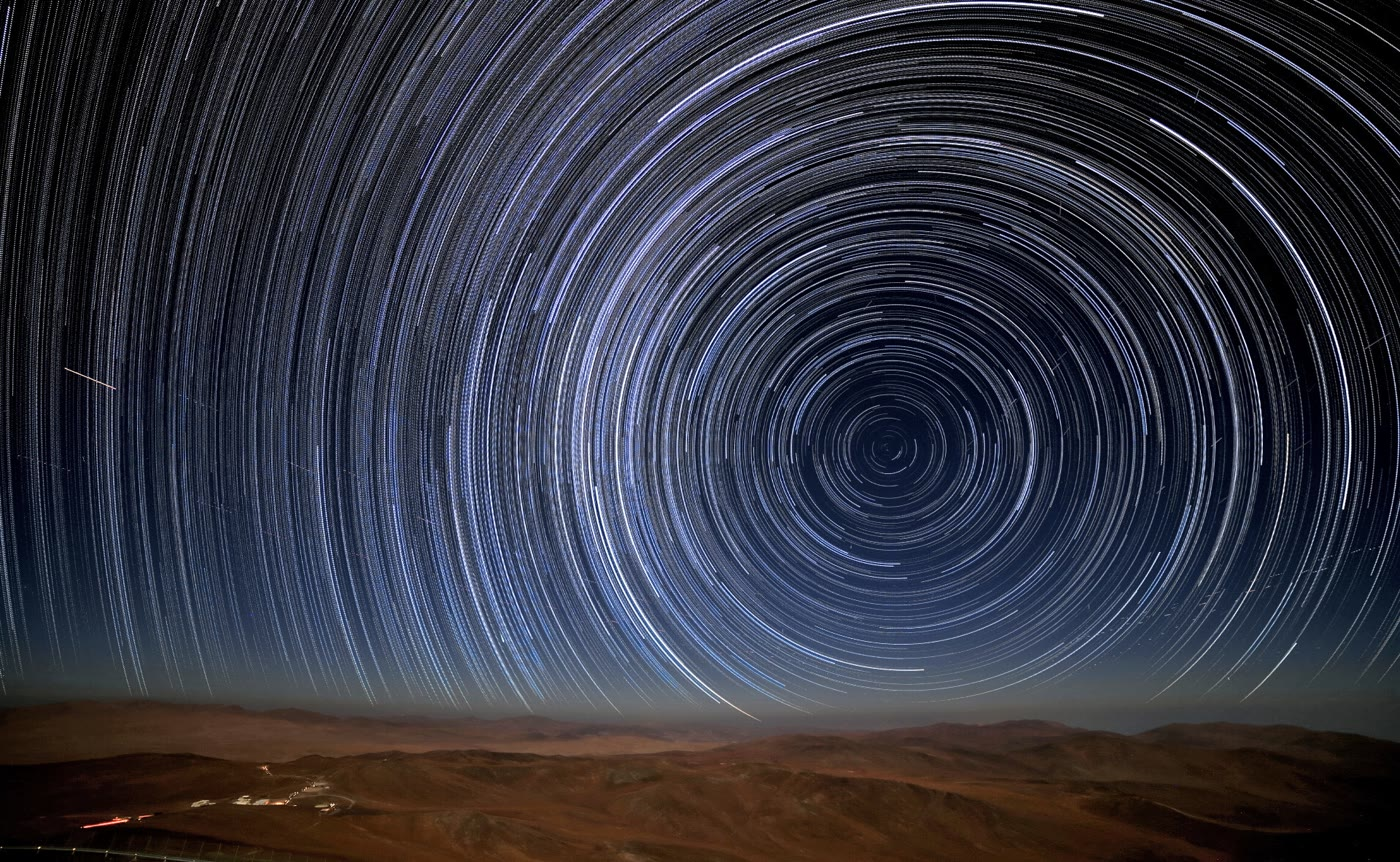
\includegraphics[width=0.8\linewidth]{images/book3/b1-star-trails-paranal.jpg}
% ledger: commons:eso-paranal-star-trails, mpc:paranal

{\small 帕拉纳尔天文台上空的星迹，位于阿塔卡马沙漠，
南纬 \ang{24.6}。长时间曝光记录了每颗恒星绕
南\omterm{def:b1:spherical-astronomy:celestial-sphere}{天极}的弧线，南\omterm{def:b1:spherical-astronomy:celestial-sphere}{天极}高出南方地平线 \ang{24.6}。
照片：R.~Wesson/ESO, CC BY 4.0。}
\end{omfigure}

\section{恒星时与太阳时}

\begin{definition}[黄道]\label{def:b1:spherical-astronomy:ecliptic}
\emph{黄道}\index{黄道}是\omterm{def:b1:spherical-astronomy:celestial-sphere}{天球}上太阳一年中视运动所沿的\omterm{def:b1:spherical-astronomy:spherical-triangle}{大圆}，
即地球轨道面在\omterm{def:b1:spherical-astronomy:celestial-sphere}{天球}上的迹线。
它与\omterm{def:b1:spherical-astronomy:celestial-sphere}{天赤道}的夹角称为
\emph{黄赤交角}\index{黄赤交角}
$\varepsilon$，即地轴相对于轨道面的倾角。黄道
与赤道相交于两点；\emph{春分
点}\index{春分点} $\gamma$ 是太阳每年三月
由南向北穿过赤道的那一点。太阳的黄经 $\lambda_\odot$
是沿黄道自 $\gamma$ 向东量取的角。
\end{definition}

% ledger: earth:obliquity (23.44)
今日的\omterm{def:b1:spherical-astronomy:ecliptic}{黄赤交角}为 $\varepsilon = \ang{23.44}$。

\begin{definition}[恒星时]\label{def:b1:spherical-astronomy:sidereal-time}
当地\emph{恒星时}\index{恒星时}是
\omterm{def:b1:spherical-astronomy:ecliptic}{春分点} $\gamma$ 的\omterm{def:b1:spherical-astronomy:equatorial}{时角}。恒星日是相继两次
$\gamma$ 经过子午线之间的时间间隔。
\end{definition}

由于\omterm{def:b1:spherical-astronomy:equatorial}{赤经}自 $\gamma$ 向东量取，
\omterm{def:b1:spherical-astronomy:equatorial}{时角}自子午线向西量取，对任一恒星有
\[
  H = \mathrm{LST} - \alpha ,
\]
其中 LST 为当地\omterm{def:b1:spherical-astronomy:sidereal-time}{恒星时}：恒星过子午线时，
当地\omterm{def:b1:spherical-astronomy:sidereal-time}{恒星时}恰等于其\omterm{def:b1:spherical-astronomy:equatorial}{赤经}。天文台上显示\omterm{def:b1:spherical-astronomy:sidereal-time}{恒星时}的时钟
一眼即可看出天空中哪一部分正位于头顶。

\begin{proposition}[恒星日与太阳日]\label{prop:b1:spherical-astronomy:sidereal-day}
在 $N$ 个平太阳日构成的一个\omterm{def:b1:spherical-astronomy:tropical-year}{回归年}中，地球相对于恒星自转 $N + 1$ 圈。
因此恒星日的长度为
\[
  \frac{N}{N + 1}\times\qty{24}{h},
\]
取 $N = 365.2422$ 时，该值为 \qty{23}{h}~\qty{56}{min}~\qty{4.09}{s}：
恒星每日过子午线的时刻，按\omterm{def:b1:spherical-astronomy:solar-time}{平太阳时}计，
比前一天早 \qty{3}{min}~\qty{56}{s}。
\end{proposition}

\begin{proof}
% ledger: usno:tropical-year, earth:Trot (23.9345 h)
在一年内分别相对于太阳和恒星计数自转圈数。
太阳一年沿\omterm{def:b1:spherical-astronomy:ecliptic}{黄道}向东绕行一周，方向与
地球自转方向相同。相对于太阳，地球因此比相对于恒星少自转一圈，
即 $N$ 个太阳日与 $N + 1$ 个恒星日恰好填满同一年。
恒星日为太阳日的 $N/(N+1)$，即
$\qty{86400}{s}\times 365.2422/366.2422 = \qty{86164.09}{s}$；两者之差为
$\qty{235.9}{s}$。这与地球相对于恒星的
实测自转周期 \qty{23.9345}{h} 相符。
\end{proof}

\begin{definition}[太阳时]\label{def:b1:spherical-astronomy:solar-time}
\emph{真太阳时}\index{真太阳时}是太阳的\omterm{def:b1:spherical-astronomy:equatorial}{时角}
加上 12 小时：日晷所示即此时刻，正午即太阳过子午线之时。
\emph{平太阳时}\index{平太阳时}是
沿\omterm{def:b1:spherical-astronomy:celestial-sphere}{天赤道}以均匀速率运动的虚构平太阳的\omterm{def:b1:spherical-astronomy:equatorial}{时角}加上 12 小时，
该平太阳每一\omterm{def:b1:spherical-astronomy:tropical-year}{回归年}绕\omterm{def:b1:spherical-astronomy:celestial-sphere}{天赤道}一周。
两者之差，即真太阳时减平太阳时，称为
\emph{时差}\index{时差}。
\end{definition}

真太阳相对平太阳有时超前、有时落后，原因有两个。
地球在近日点（约一月初）附近运动比在远日点附近快，
因此太阳沿\omterm{def:b1:spherical-astronomy:ecliptic}{黄道}的视运动不均匀（开普勒第二定律）；
另外，太阳沿\omterm{def:b1:spherical-astronomy:ecliptic}{黄道}运动，而\omterm{def:b1:spherical-astronomy:ecliptic}{黄道}与赤道有夹角，
因此即使沿\omterm{def:b1:spherical-astronomy:ecliptic}{黄道}的运动是均匀的，它投影到赤道上——即\omterm{def:b1:spherical-astronomy:equatorial}{时角}所度量的量——
也不均匀，在至点附近比在分点附近快。
民用时钟按其时区参考子午线上的\omterm{def:b1:spherical-astronomy:solar-time}{平太阳时}计时；
\omterm{def:b1:spherical-astronomy:geographic}{经度}为 $\lambda$ 处的地方\omterm{def:b1:spherical-astronomy:solar-time}{平太阳时}，比格林尼治时间早
$\lambda/\ang{15}$ 小时。

\begin{omfigure}
\begin{tikzpicture}
\begin{axis}[omrecord, width=0.9\linewidth, height=5.2cm, xmin=0, xmax=365,
  xtick={0,31,59,90,120,151,181,212,243,273,304,334,365},
  xticklabels={1月,2月,3月,4月,5月,6月,7月,8月,9月,10月,11月,12月,},
  ylabel={时差（分）}, ymin=-20, ymax=21,
  tick label style={font=\scriptsize}, label style={font=\small}]
\addplot[black!50, line width=0.4pt] coordinates {(0,0) (365,0)};
\addplot[omDef, line width=1.1pt] table[x=day, y=eot_min] {figdata/out/bachelor-1-day_length-eot.dat};
\node[font=\scriptsize, above, fill=white, inner sep=1pt] at (axis cs:306,16.6) {$+16.4$};
\node[font=\scriptsize, below, fill=white, inner sep=1pt] at (axis cs:41,-14.4) {$-14.2$};
\end{axis}
\end{tikzpicture}

{\small 全年的\omterm{def:b1:spherical-astronomy:solar-time}{时差}曲线（\omterm{def:b1:spherical-astronomy:solar-time}{真太阳时}减\omterm{def:b1:spherical-astronomy:solar-time}{平太阳时}）：
日晷在 11 月初最多快 \qty{16.4}{min}，
在 2 月中旬最多慢 \qty{14.2}{min}。计算采用开普勒轨道，
偏心率 0.0167，\omterm{def:b1:spherical-astronomy:ecliptic}{黄赤交角} \ang{23.44}，近日点\omterm{def:b1:spherical-astronomy:geographic}{经度}
及 2026 年 3 月春分日期。}
% ledger: earth:ecc, earth:obliquity, nasa:earth-perihelion-longitude, usno:seasons-2026
\end{omfigure}

\section{升落与太阳}

\begin{proposition}[升落]\label{prop:b1:spherical-astronomy:rising}
在\omterm{def:b1:spherical-astronomy:geographic}{纬度} $\varphi$ 处，\omterm{def:b1:spherical-astronomy:equatorial}{赤纬}为 $\delta$ 且有升落的恒星，
在\omterm{def:b1:spherical-astronomy:equatorial}{时角} $\pm H_0$ 处穿过地平线，其中
\[
  \cos H_0 = -\tan\varphi\tan\delta ,
\]
\omterm{def:b1:spherical-astronomy:horizontal}{方位角}为 $\mathrm{A}_0$，其中 $\cos\mathrm{A}_0 = \sin\delta/\cos\varphi$
（升起时；降落时\omterm{def:b1:spherical-astronomy:horizontal}{方位角}为 $\ang{360} - \mathrm{A}_0$）。它在地平线以上的时间为
按每小时 \ang{15} 换算为小时数的 $2H_0$。
\end{proposition}

\begin{proof}
在地平线上 $h = 0$，由\cref{prop:b1:spherical-astronomy:transform}得
$0 = \sin\varphi\sin\delta + \cos\varphi\cos\delta\cos H_0$，又
$\cos\mathrm{A}_0 = \sin\delta/\cos\varphi$。\omterm{def:b1:spherical-astronomy:equatorial}{时角}以
每小时 \ang{15} 的速率均匀增加，从升起时的 $-H_0$ 增至降落时的 $+H_0$。
\end{proof}

对太阳而言，若将太阳视为一个点，
并忽略大气对光线的折射（两者都会使白昼增加几分钟），
由此即可得白昼长度。在春分日 $\delta = 0$，$H_0 = \ang{90}$：昼夜
各地均为十二小时，太阳正东升起。

\begin{omfigure}
\begin{tikzpicture}
\begin{axis}[omrecord, width=0.85\linewidth, height=5.6cm, xmin=40, xmax=320, ymin=0, ymax=75,
  xtick={45,90,135,180,225,270,315}, xticklabels={东北, 东, 东南, 南, 西南, 西, 西北}, ytick={0,15,30,45,60,75},
  xlabel={方位角}, ylabel={太阳高度角（$^\circ$）},
  tick label style={font=\scriptsize}, label style={font=\small}]
\addplot[omThm, line width=1pt] table[x=az_deg, y=alt_deg] {figdata/out/bachelor-1-sun_paths-june.dat};
\addplot[black, line width=1pt] table[x=az_deg, y=alt_deg] {figdata/out/bachelor-1-sun_paths-equinox.dat};
\addplot[omDef, line width=1pt] table[x=az_deg, y=alt_deg] {figdata/out/bachelor-1-sun_paths-december.dat};
\begin{scope}[font=\scriptsize, fill=white, fill opacity=0.8, text opacity=1, inner sep=1pt]
  \node[omThm, above, fill=white] at (axis cs:180,68.4) {六月至点，$\ang{68.4}$};
  \node[above, fill=white] at (axis cs:180,45) {分点，$\ang{45}$};
  \node[omDef, above, fill=white] at (axis cs:180,21.6) {十二月至点，$\ang{21.6}$};
\end{scope}
\end{axis}
\end{tikzpicture}

{\small 北纬 \ang{45} 处，六月至点时太阳在天空中的路径（红色）、
分点（黑色）及十二月至点（蓝色）时的路径，其中
正午高度角为 $\ang{90} - \varphi + \delta_\odot$。春分日
太阳正东升起、正西落下；六月时太阳在东北方升起。}
\end{omfigure}

\begin{proposition}[太阳的赤纬]\label{prop:b1:spherical-astronomy:sun-declination}
太阳位于黄经 $\lambda_\odot$ 时，其\omterm{def:b1:spherical-astronomy:equatorial}{赤纬}与
\omterm{def:b1:spherical-astronomy:equatorial}{赤经}满足：
\[
  \sin\delta_\odot = \sin\varepsilon\sin\lambda_\odot, \qquad
  \tan\alpha_\odot = \cos\varepsilon\tan\lambda_\odot .
\]
\end{proposition}

\begin{proof}
取坐标轴，使 $x$ 指向 $\gamma$，$z$ 指向北\omterm{def:b1:spherical-astronomy:celestial-sphere}{天极}。
在与\omterm{def:b1:spherical-astronomy:ecliptic}{黄道}固连的坐标系 $x$、$y'$、$z'$ 中，$z'$ 指向黄极，
太阳方向为 $(\cos\lambda_\odot, \sin\lambda_\odot, 0)$。
\omterm{def:b1:spherical-astronomy:ecliptic}{黄道}坐标轴由赤道坐标轴转过角 $\varepsilon$ 所得，转轴为
$x$ 轴，因此在赤道坐标系中，太阳方向为
$(\cos\lambda_\odot,\ \sin\lambda_\odot\cos\varepsilon,\
\sin\lambda_\odot\sin\varepsilon)$。其 $z$ 分量为 $\sin\delta_\odot$；
$y$ 分量与 $x$ 分量之比为 $\tan\alpha_\odot$。
\end{proof}

\begin{omfigure}
\begin{tikzpicture}
\begin{axis}[omrecord, width=0.9\linewidth, height=6cm, xmin=0, xmax=365, ymin=0, ymax=24,
  xtick={0,31,59,90,120,151,181,212,243,273,304,334,365},
  xticklabels={1月,2月,3月,4月,5月,6月,7月,8月,9月,10月,11月,12月,}, ytick={0,6,12,18,24},
  ylabel={昼长 (h)}, tick label style={font=\scriptsize}, label style={font=\small},
  legend style={font=\scriptsize, at={(0.5,1.02)}, anchor=south, draw=none}, legend columns=5,
  legend cell align=left]
\addplot[black, line width=0.9pt] table[x=day, y=lat0] {figdata/out/bachelor-1-day_length-lengths.dat};
\addplot[omDef, line width=0.9pt] table[x=day, y=lat30] {figdata/out/bachelor-1-day_length-lengths.dat};
\addplot[omThm, line width=0.9pt] table[x=day, y=lat45] {figdata/out/bachelor-1-day_length-lengths.dat};
\addplot[omField, line width=0.9pt] table[x=day, y=lat60] {figdata/out/bachelor-1-day_length-lengths.dat};
\addplot[black, line width=0.9pt, densely dashed] table[x=day, y=lat70] {figdata/out/bachelor-1-day_length-lengths.dat};
\legend{\ang{0}, \ang{30} 北, \ang{45} 北, \ang{60} 北, \ang{70} 北}
\end{axis}
\end{tikzpicture}

{\small 五个北纬\omterm{def:b1:spherical-astronomy:geographic}{纬度}处全年的昼长（太阳中心位于几何地平线之上），
由
\cref{prop:b1:spherical-astronomy:rising,prop:b1:spherical-astronomy:sun-declination}得出。
在北纬 \ang{70}，六月至点前后太阳连续数周不落，
十二月至点前后太阳则整日不出。南半球的曲线
相差半年。}
\end{omfigure}

\begin{definition}[日射量]\label{def:b1:spherical-astronomy:insolation}
某地某时刻的\emph{日射量}\index{日射量}，是
大气顶部水平面单位面积上接收到的太阳光功率。
设 $S_0$ 为太阳在平均距离 $a$ 处的太阳辐照度，
$r$ 为实际距离，$\theta_z$ 为太阳\omterm{def:b1:spherical-astronomy:celestial-sphere}{天顶}距，则
\[
  I = S_0\left(\frac{a}{r}\right)^{2}\cos\theta_z = S_0\left(\frac{a}{r}\right)^{2}\sin h_\odot
  \quad (h_\odot > 0), \qquad I = 0 \text{ 夜间}.
\]
\end{definition}

% ledger: earth:TSI (1361 W/m2), earth:peri, earth:aph, earth:a
因子 $(a/r)^2$ 是光的平方反比律（见物理各册）；
因子 $\cos\theta_z$ 的出现，是因为截面为一平方米的光束，
会铺展到 $1/\cos\theta_z$ 平方米的水平地面上。取
$S_0 = \qty{1361}{W.m^{-2}}$，日地距离在近日点时为
\qty{147.1e6}{km}、远日点时为\qty{152.1e6}{km}，则因子
$(a/r)^2$ 全年变化幅度为 $\pm\qty{3.4}{\percent}$。地轴的倾斜作用要大得多：
它同时改变正午高度角和昼长，二者共同造成了季节。
\omterm{def:b1:spherical-astronomy:insolation}{日射量}的逐日与逐年累积量驱动着气候，
这些量将在
\cref{ch:b1:radiation-heat-transport}中计算。


\section{历法}

\begin{definition}[回归年]\label{def:b1:spherical-astronomy:tropical-year}
\emph{回归年}\index{回归年}是太阳相继两次
经过\omterm{def:b1:spherical-astronomy:ecliptic}{春分点}的平均时间间隔。它决定季节，
其长度为 365.2422 个平均太阳日。
\end{definition}

% ledger: usno:tropical-year, earth:Psid (365.256 d)
\omterm{def:b1:spherical-astronomy:tropical-year}{回归年}比恒星年短约二十分钟，这里的恒星年
即地球回到恒星背景中同一位置所需的时间
（365.256 天）。这是因为地球的自转轴缓慢转动——即岁差——，
使\omterm{def:b1:spherical-astronomy:ecliptic}{春分点}沿\omterm{def:b1:spherical-astronomy:ecliptic}{黄道}向西移动（见本科二年级分册）。
历法必须使整数个日数与\omterm{def:b1:spherical-astronomy:tropical-year}{回归年}相配，
以使季节在相同的日期重现。

\begin{proposition}[格里高利历的年长]\label{prop:b1:spherical-astronomy:gregorian}
在格里高利历中，年份数能被 4 整除的年为闰年，长 366 天；
但世纪年只有能被
400 整除时才是闰年。其平均年长为
\[
  365 + \frac14 - \frac1{100} + \frac1{400} = \num{365.2425}\text{ 天},
\]
它相对于季节漂移，约每 3300 年漂移一天。
\end{proposition}

\begin{proof}
% ledger: usno:leap-rule, usno:tropical-year
400 年中能被 4 整除的年有 100 个，其中包括
四个世纪年，其中三个不能被 400 整除。因此共有 97 个闰年，
共 $400\times 365 + 97 = 146\,097$ 天，
即平均每年 365.2425 天。与\omterm{def:b1:spherical-astronomy:tropical-year}{回归年}的 365.2422 天相比，
每年多出 0.0003 天：约 $1/0.0003 \approx 3300$ 年多出一天。
\end{proof}

\begin{history}[1582 年的历法改革]
% ledger: usno:gregorian-1582
儒略历源自罗马，每四年增加一个闰日，
其年长 365.25 天，比\omterm{def:b1:spherical-astronomy:tropical-year}{回归年}长 0.0078 天，
即每 128 年多出一天。经过数个世纪，春分日的日期
逐渐偏离 3 月 21 日，而该日期正是复活节推算所依据的日期。
1582 年，教皇格里高利十三世颁行了以其名字命名的历法，
一次性去掉了累积的多余日数，并以
\cref{prop:b1:spherical-astronomy:gregorian}中的规则取代儒略历的规则。
它已成为国际通用的民用历法。
\end{history}

\begin{inthefield}[从星象确定位置]
在卫星定位出现之前，航海者在海上依靠天象确定\omterm{def:b1:spherical-astronomy:geographic}{纬度}与\omterm{def:b1:spherical-astronomy:geographic}{经度}。
他们用六分仪测量正午太阳的高度，或黄昏时两三颗恒星的高度，
并从按格林尼治子午线走时的天文钟上读出时刻。
每个高度，连同该恒星的\omterm{def:b1:spherical-astronomy:equatorial}{赤纬}及历书给出的格林尼治\omterm{def:b1:spherical-astronomy:equatorial}{时角}，
确定地球上的一个\omterm{def:b1:spherical-astronomy:spherical-triangle}{小圆}，即恒星恰好处于该高度的点的集合，
船位于其上。两个或三个这样的\omterm{def:b1:spherical-astronomy:spherical-triangle}{小圆}相交于船的位置——
这是航海者每天在海上完成的球面三角计算。
仅凭太阳的正午高度即可求得\omterm{def:b1:spherical-astronomy:geographic}{纬度}
（\cref{prop:b1:spherical-astronomy:culmination}）；
当地正午的钟面时刻则给出\omterm{def:b1:spherical-astronomy:geographic}{经度}，
每度相当于 4 分钟时间。
\begin{center}

\includegraphics[width=0.55\linewidth]{images/book3/ai/b1-sextant.jpg}
\end{center}
\end{inthefield}

\section{练习}

\begin{exercise}[$\star$]\label{exo:b1:spherical-astronomy:1}
观测者位于北纬 \ang{52}，北\omterm{def:b1:spherical-astronomy:celestial-sphere}{天极}的高度为多少？
按\omterm{def:b1:spherical-astronomy:equatorial}{赤纬}判断，哪些恒星在该处永不落下，
哪些永不升起？
\end{exercise}

\begin{exercise}[$\star$]\label{exo:b1:spherical-astronomy:2}
将\omterm{def:b1:spherical-astronomy:equatorial}{赤经} \qty{6}{h}~\qty{45}{min} 换算为度。
当地\omterm{def:b1:spherical-astronomy:sidereal-time}{恒星时}为 \qty{10}{h}~\qty{0}{min} 时，\omterm{def:b1:spherical-astronomy:equatorial}{赤经}为该值的恒星的\omterm{def:b1:spherical-astronomy:equatorial}{时角}是多少？
该恒星位于子午线的东侧还是西侧？
\end{exercise}

\begin{exercise}[$\star$]\label{exo:b1:spherical-astronomy:3}
在北纬 \ang{40}，
计算正午时太阳在两个至日和两个分日的高度（$\varepsilon = \ang{23.44}$）。
\end{exercise}

\begin{exercise}[$\star$]\label{exo:b1:spherical-astronomy:4}
1900 年是闰年吗？2000 年呢？2100 年将是闰年吗？
相对于\omterm{def:b1:spherical-astronomy:tropical-year}{回归年} 365.2422 天，儒略历每个世纪漂移多少天？
格里高利历每个世纪漂移多少天？
\end{exercise}

\begin{exercise}[$\star\star$]\label{exo:b1:spherical-astronomy:5}
两点位于北纬 \ang{45}，\omterm{def:b1:spherical-astronomy:geographic}{经度}分别为 \ang{0} 与
东经 \ang{90}。计算两点之间的\omterm{def:b1:spherical-astronomy:spherical-triangle}{大圆}距离
（$R = \qty{6371}{km}$）以及沿纬线的距离。
哪一个较短？短多少？
\end{exercise}

\begin{exercise}[$\star\star$]\label{exo:b1:spherical-astronomy:6}
在北纬 \ang{48}，\omterm{def:b1:spherical-astronomy:equatorial}{赤纬}为 \ang{20} 的恒星，其\omterm{def:b1:spherical-astronomy:equatorial}{时角}为
\ang{30}。计算其高度与\omterm{def:b1:spherical-astronomy:horizontal}{方位角}。
观测者应朝哪个方向观察？
\end{exercise}

\begin{exercise}[$\star\star$]\label{exo:b1:spherical-astronomy:7}
计算北纬 \ang{60}，在六月至日时的白昼长度，
将太阳视为几何地平线上的一个点。
用日长图核对你的结果。
\end{exercise}

\begin{exercise}[$\star\star$]\label{exo:b1:spherical-astronomy:8}
某恒星今晚于当地平均时 22:00 过子午线。30 天后它将于何时过子午线？
它在正午过子午线还需多少天，
此时因白昼而不可见？
\end{exercise}

\begin{exercise}[$\star\star$]\label{exo:b1:spherical-astronomy:9}
计算正午时大气层顶部的\omterm{def:b1:spherical-astronomy:insolation}{日射量}，\omterm{def:b1:spherical-astronomy:geographic}{纬度}为北纬
\ang{45}：(a) 在分日，取 $r = a$；(b) 在六月至日，
取 $r$ 为远日点距离。数据：$S_0 = \qty{1361}{W.m^{-2}}$，
$a = \qty{149.598e6}{km}$，远日点为 \qty{152.100e6}{km}。
\end{exercise}

\begin{exercise}[$\star\star\star$]\label{exo:b1:spherical-astronomy:10}
利用\cref{prop:b1:spherical-astronomy:sun-declination}，计算
太阳黄经为 \ang{60} 时太阳的\omterm{def:b1:spherical-astronomy:equatorial}{赤纬}与\omterm{def:b1:spherical-astronomy:equatorial}{赤经}，
\omterm{def:b1:spherical-astronomy:equatorial}{赤经}比黄经落后多少度？据此结果，
说明\omterm{def:b1:spherical-astronomy:ecliptic}{黄道}倾角为何会对
\omterm{def:b1:spherical-astronomy:solar-time}{时差}产生影响。
\end{exercise}

\begin{exercise}[$\star\star\star$]\label{exo:b1:spherical-astronomy:11}
证明在六月至日，太阳于\omterm{def:b1:spherical-astronomy:horizontal}{方位角} $\mathrm{A}_0$ 处升起，
其中 $\cos\mathrm{A}_0 = \sin\varepsilon/\cos\varphi$。在哪一\omterm{def:b1:spherical-astronomy:geographic}{纬度}，
太阳恰好在东北方升起？该公式在\omterm{def:b1:spherical-astronomy:geographic}{纬度}
超过 $\ang{90} - \varepsilon$ 时会怎样？
\end{exercise}

\begin{exercise}[$\star\star\star$]\label{exo:b1:spherical-astronomy:12}
月形是球面上连接两个相对点的两个半\omterm{def:b1:spherical-astronomy:spherical-triangle}{大圆}之间的部分，
两半\omterm{def:b1:spherical-astronomy:spherical-triangle}{大圆}之间的夹角为 $\theta$。(a) 证明其面积为
$2\theta R^2$。(b) \omterm{def:b1:spherical-astronomy:spherical-triangle}{球面三角形} $ABC$ 的每条边延长为完整\omterm{def:b1:spherical-astronomy:spherical-triangle}{大圆}后，
与其余两边共同给出三对相对月形，其角分别为 $A$、$B$、$C$，
它们覆盖整个球面，三角形及其对顶三角形
各被覆盖三次。由此推出吉拉德定理：三角形面积为
$R^2(A + B + C - \pi)$。(c) 将其应用于三个角均为直角的三角形，
以及本章中所画的三角形（角分别为 \ang{89.9}、\ang{64.9}、
\ang{67.4}）。
\end{exercise}

\section{问题：山地天文台的一夜}

\begin{problem}[{周末问题——帕拉纳尔天文台位于何处，
其天空呈现什么景象，以及其最长夜晚持续多久}]
\label{pb:b1:spherical-astronomy:1}
% ledger: mpc:paranal, mpc:greenwich, simbad:sirius, simbad:canopus, usno:seasons-2026, earth:obliquity, usno:tropical-year
% numbers computed in the scratch calculator calc/ch01.py from the rounded data
帕拉纳尔天文台位于阿塔卡马沙漠，\omterm{def:b1:spherical-astronomy:geographic}{纬度}为
南纬 \ang{24.63}，\omterm{def:b1:spherical-astronomy:geographic}{经度}为西经 \ang{70.40}。皇家格林尼治天文台
\omterm{def:b1:spherical-astronomy:geographic}{经度}由其起算，位于北纬 \ang{51.48}，\omterm{def:b1:spherical-astronomy:geographic}{经度} \ang{0.00}。南天两颗明亮的
恒星的坐标如下：
\begin{center}
\small
\begin{tabular}{lcc}
\hline
恒星 & \omterm{def:b1:spherical-astronomy:equatorial}{赤经} & \omterm{def:b1:spherical-astronomy:equatorial}{赤纬} \\
\hline
天狼星 & \qty{6}{h}~\qty{45}{min}~\qty{9}{s} & \ang{-16.72} \\
老人星 & \qty{6}{h}~\qty{23}{min}~\qty{57}{s} & \ang{-52.70} \\
\hline
\end{tabular}
\end{center}
取 $R = \qty{6371}{km}$，$\varepsilon = \ang{23.44}$，\omterm{def:b1:spherical-astronomy:tropical-year}{回归年}为
365.2422 天，并将太阳视为几何地平线上的一个点。

\medskip
\noindent\textbf{第一部分——地球仪上的帕拉纳尔。}
\begin{enumerate}
  \item 求帕拉纳尔和格林尼治的余纬，以及它们的
        \omterm{def:b1:spherical-astronomy:geographic}{经度}差。
  \item 写出三角形北极–帕拉纳尔–格林尼治的球面余弦定理，
        并计算两座天文台之间的角距离 $\Delta$ 的
        余弦。
  \item 由此求出以度表示的 $\Delta$，以及
        以千米表示的\omterm{def:b1:spherical-astronomy:spherical-triangle}{大圆}距离。
  \item 计算从帕拉纳尔指向格林尼治的初始航向
        （见\cref{met:b1:spherical-astronomy:great-circle}）。
  \item 用球面正弦定理检验该航向。
  \item 若飞机全程保持这一航向，能否到达格林尼治？
        说明理由。
\end{enumerate}

\medskip
\noindent\textbf{第二部分——帕拉纳尔的天空。}
\begin{enumerate}[resume]
  \item 南\omterm{def:b1:spherical-astronomy:celestial-sphere}{天极}在帕拉纳尔的南方地平线
        上方多高？
  \item 天狼星经过子午圈时的高度是多少，它位于
        \omterm{def:b1:spherical-astronomy:celestial-sphere}{天顶}的哪一侧？
  \item 在帕拉纳尔，\omterm{def:b1:spherical-astronomy:equatorial}{赤纬}低于多少的恒星是\omterm{def:b1:spherical-astronomy:circumpolar}{拱极星}？老人星
        是\omterm{def:b1:spherical-astronomy:circumpolar}{拱极星}吗？
  \item 老人星能达到的最大高度是多少？
  \item 计算天狼星升起时的\omterm{def:b1:spherical-astronomy:equatorial}{时角}，以及它在地平线
        以上停留的时间（以\omterm{def:b1:spherical-astronomy:sidereal-time}{恒星时}小时计）。
  \item 天狼星在何\omterm{def:b1:spherical-astronomy:horizontal}{方位角}升起？
\end{enumerate}

\medskip
\noindent\textbf{第三部分——时钟。}
\begin{enumerate}[resume]
  \item 天狼星经过子午圈时的地方\omterm{def:b1:spherical-astronomy:sidereal-time}{恒星时}是多少？
  \item 计算恒星日的长度，以及每晚恒星经过子午圈
        的时刻提前多少分钟。
  \item 取三月春分（2026 年 3 月 20 日）地方平子夜的
        地方\omterm{def:b1:spherical-astronomy:sidereal-time}{恒星时}为 \qty{12}{h}，此时太阳接近\omterm{def:b1:spherical-astronomy:ecliptic}{春分点}；
        此后每天增加 $24/365.2422$ 小时。
        天狼星在地方平子夜经过子午圈的时刻，
        是春分后的第几天？是哪一天？
  \item 当夜，帕拉纳尔的地方平时与
        格林尼治时间相差多少？
  \item 此时\omterm{def:b1:spherical-astronomy:solar-time}{时差}约为 \qty{-3}{min}。天狼星经过子午圈时，
        天文台的日晷所示的时刻（\omterm{def:b1:spherical-astronomy:solar-time}{真太阳时}）
        是多少？
  \item 一周后，天狼星经过子午圈的时刻提前多少？
\end{enumerate}

\medskip
\noindent\textbf{第四部分——最长的夜晚。}
\begin{enumerate}[resume]
  \item 两个至日时太阳的\omterm{def:b1:spherical-astronomy:equatorial}{赤纬}各是多少？
  \item 计算帕拉纳尔在六月和十二月至日的
        正午太阳高度。十二月时它位于\omterm{def:b1:spherical-astronomy:celestial-sphere}{天顶}的哪一侧？
  \item 十二月至日时，日地距离是平均距离的 0.9837 倍。
        计算帕拉纳尔上空大气层顶部正午的
        \omterm{def:b1:spherical-astronomy:insolation}{日射量}（$S_0 = \qty{1361}{W.m^{-2}}$）。
  \item 帕拉纳尔的夜晚在哪个至日最长？计算该日
        日落时的\omterm{def:b1:spherical-astronomy:equatorial}{时角}。
  \item 该日太阳在何\omterm{def:b1:spherical-astronomy:horizontal}{方位角}升起？
  \item 推算帕拉纳尔一年中最长夜晚的长度，
        以小时和分钟表示。
\end{enumerate}
\end{problem}
